\documentclass{article}
\usepackage{amsmath}
\usepackage{amssymb}
\usepackage[a4paper, top=25mm, bottom=25mm, left=25mm, right=25mm]{geometry}
\usepackage{pgfplots}
\usepackage{mathtools}
\pgfplotsset{compat=1.18}
\usepgfplotslibrary{polar}

\begin{document}
\pagestyle{empty}
\large

\begin{center}
2011-2012 Spring \\MAT124 Midterm I\\(28/03/2012)\\Time: 13:00 - 15:00\\Duration: 120 minutes
\end{center}

\noindent 1. Consider the curve with the polar equations $r=2-2\sin\theta$.

\hfill

(a) Sketch this curve.

\hfill

(b) Find the area of the region enclosed by this curve.

\hfill

(c) Find the tangent vector(s) to this curve at $\displaystyle\theta=\frac\pi4$.

\hfill

\noindent 2. Consider the points $A(0,-1,1),\:B(-1,0,1),\:C(1,0,2),\:D(0,0,1)$  in $\mathbb{R}^3$.

\hfill

(a) Find the equation of the plane passing through $A, B$ and $C$.

\hfill

(b) Find the distance from the point $D$ to the plane passing through $A, B$ and $C$.

\hfill

(c) Find the equation of the line passing through $B$ and $D$.

\hfill

\noindent 3. Consider the space curve whose vector equation is given by

\[r(t)=\mathrm{e}^t\sin t\,\mathbf{i}+\mathrm{e}^t\cos t\,\mathbf{j}+\mathrm{e}^t\,\mathbf{k} \quad\text{for}\quad 0\leq t\leq1\,.\]

\hfill

(a) Sketch the curve.

\hfill

(a) Find the length of the curve.

\hfill

\noindent 4. Evaluate the limit, if it exists, and explain your answer.

\hfill

(a) $\displaystyle \lim_{(x,y)\to(-1,-2)}\frac{y+2}{x^2y-xy+2x^2-2x}$ \ \ \ (b) $\displaystyle\lim_{(x,y)\to(0,0)}\frac{4x^2y}{x^4+y^2}$

\hfill

\hfill

\noindent 5. Answer each independent question below.

\hfill

(a) Let $f(x,y)=\ln\left(x^2+y^2\right)$. Evaluate $f_{xx}+f_{yy}$.

\hfill

(b) Sketch the surface given by $z=2x^2+y^2+4y+6$.

\newpage

\begin{center}
2011-2012 Spring Midterm I (28/03/2012) Solutions\\
(Last update: 28/08/2025 14:01)
\end{center}

\noindent 1.

\hfill

\noindent (a)
\begin{center}
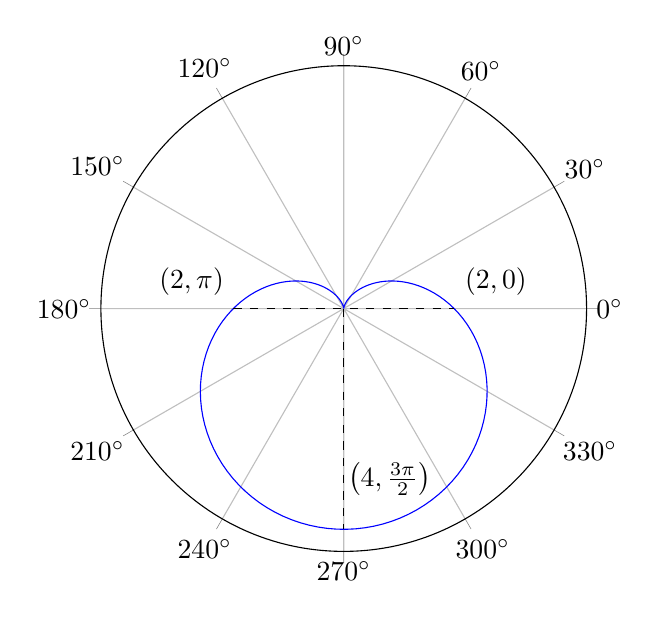
\begin{tikzpicture}
  \begin{polaraxis}[ytick=\empty, axis y line=none, xticklabel=$\pgfmathprintnumber{\tick}^\circ$, scale=0.9]
    \addplot [
      domain=0:2*pi,
      samples=150,
      blue,
      data cs=polarrad,
    ] {2-2*sin(deg(x))};

    \draw[dashed] (axis cs: 0,-2) -- (axis cs: 0,2);
    \node at (axis cs: -10,-2.8) {$(2,\pi)$};
    \node at (axis cs: 10,2.8) {$(2,0)$};
    \node at (axis cs: 285,3.2) {$\left(4,\frac{3\pi}2\right)$};
    \draw[dashed] (axis cs: 0,0) -- (axis cs: 270,4);

  \end{polaraxis}
\end{tikzpicture}
\end{center}

\noindent (b)
\begin{align*}A&=\frac12\int_a^br^2\,d\theta=\frac12\int_0^{2\pi}\left(2-2\sin\theta\right)^2\,d\theta=\frac12\int_0^{2\pi}\left(4-8\sin\theta+4\sin^2\theta\right)\,d\theta\\\\&=\frac12\int_0^{2\pi}\left(4-8\sin\theta+4\sin^2\theta\right)\,d\theta=\int_0^{2\pi}\left(2-4\sin\theta+1-\cos2\theta\right)\,d\theta\\\\&=\left[2\theta+4\cos\theta+\theta-\frac12\sin2\theta\right]_0^{2\pi}=\left[\left(4\pi+4+2\pi\right)-(4)\right]=\boxed{6\pi}\end{align*}

\hfill

\noindent (c) The slope of the tangent line in terms of $r$ and $\theta$ is

\[\left.\frac{dy}{dx}\right|_{(r,\theta)}=\frac{f'(\theta)\cdot\sin\theta+f(\theta)\cdot\cos\theta}{f'(\theta)\cdot\cos\theta-f(\theta)\cdot\sin\theta}\]

\[f(\theta)=2-2\sin\theta, \quad f'(\theta)=-2\cos\theta\]

\[\frac{dy}{dx}=\frac{-2\cos\theta\cdot\sin\theta+(2-2\sin\theta)\cdot\cos\theta}{-2\cos\theta\cdot\cos\theta-(2-2\sin\theta)\cdot\sin\theta}=\frac{-2\sin2\theta+2\cos\theta}{-\sin2\theta-2\sin\theta+2\sin^2\theta}\]

\[\left.\frac{dy}{dx}\right|_{\left(2-\sqrt2,\:\pi/4\right)}=\frac{-2+\sqrt2}{-\sqrt2}=\sqrt2-1\]

\hfill

\noindent The tangent vectors to the curve at $\theta=\dfrac\pi4$ are

\[\boxed{\left\langle k,\:k\left(\sqrt2-1\right)\right\rangle,\quad k\in\mathbb{R}}\]

\hfill

\noindent 2. 

\hfill

\noindent (a) Choose three arbitrary points and determine the parallel vector of each of the two line segments that connect the points.

\[\overrightarrow{AB}=\left\langle-1-0,\:0-(-1),\:1-1\right\rangle=\left\langle-1,1,0\right\rangle\]
\[\overrightarrow{AC}=\left\langle1-0,\:0-(-1),\:2-1\right\rangle=\left\langle1,1,1\right\rangle\]

\hfill

\noindent The cross product of these vectors gives us the normal vector of the plane.

\begin{align*}\mathbf{n}&=\left|\begin{array}{ccc}
\mathbf{i}&\mathbf{j}&\mathbf{k}\\
-1&1&0\\
1&1&1
\end{array}\right|=\mathbf{i}\left|\begin{array}{cc}
1&0\\1&1
\end{array}\right|-\mathbf{j}\left|\begin{array}{cc}
-1&0\\1&1
\end{array}\right|+\mathbf{k}\left|\begin{array}{cc}
-1&1\\1&1
\end{array}\right|\\\\&=(1\cdot1-0\cdot1)\mathbf{i}-(-1\cdot1-0\cdot1)\mathbf{j}+(-1\cdot1-1\cdot1)\mathbf{k}=\mathbf i+\mathbf j-2\mathbf k\end{align*}

\hfill

\noindent The plane has the equation $\mathbf n\cdot\overrightarrow{PP_0}=0$. Since $C(1,0,2)$ is on the plane, the equation of the plane is

\[\boxed{1(x-1)+1(y-0)-2(z-2)=0\implies x+y-2z+3=0}\]

\hfill

\noindent (b) Let $P$ be a point on a plane, then the distance from any point $R$ to the plane is the length of the vector projection of $\overrightarrow{PR}$ onto $\mathbf n$. That is,

\[d=\left|\overrightarrow{PR}\cdot\frac{\mathbf n}{|\mathbf n|}\right|\]

\hfill

\noindent The distance from $D$ to the plane passing through $A, B, C$ can be calculated using

\[d=\left|\overrightarrow{AD}\cdot\frac{\mathbf n}{|\mathbf n|}\right|=\left|\left\langle0-0,0-(-1),1-1\right\rangle\cdot\frac{\left\langle1,1,-2\right\rangle}{\sqrt{1^2+1^2+(-2)^2}}\right|=\boxed{\frac1{\sqrt6}}\]

\noindent (c) We have

\[\mathbf{v}=\overrightarrow{BD}=\left\langle0-(-1),0-0,1-1\right\rangle=\left\langle1,0,0\right\rangle\]

\hfill

\noindent The parametric equations for a line that passes through the point $P_0(x_0,y_0,z_0)$ is given by
\[\left.\begin{array}{c}
x=x_0+v_1t\\
y=y_0+v_2t\\
z=z_0+v_3t
\end{array}\right\}\quad t\in\mathbb{R}\]

\hfill

\noindent Therefore, the parametric equations for the line passing through $B$ and $D$ is

\[\boxed{\left.\begin{array}{l}
x=-1+t\\
y=0\\
z=1
\end{array}\right\}\quad t\in\mathbb{R}}\]

\hfill 

\noindent 3.

\hfill

\noindent (a)
\begin{center}
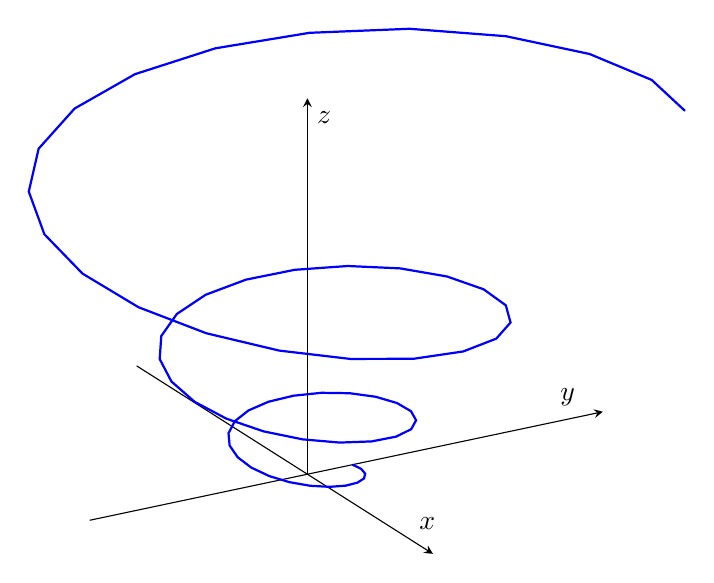
\begin{tikzpicture}
  \begin{axis}[
    view={60}{30},
    axis lines=center,
    xlabel={$x$}, ylabel={$y$}, zlabel={$z$},
    domain=0:2,
    samples=67,
    variable=t,
    xtick=\empty, ytick=\empty, ztick=\empty,
    restrict z to domain=0:7,
    scale=1.5,
  ]
    \addplot3[thick, blue] (
      {exp(t)*sin(deg(10*t))},
      {exp(t)*cos(deg(10*t))},
      {exp(t)}
    );
  \end{axis}
\end{tikzpicture}
\end{center}

\hfill

\noindent (b) The length of the parametrized curve $\mathbf{r}(t)=\left\langle x(t),\,y(t),\,z(t)\right\rangle$ for $a<t<b$ can be evaluated using the integral

\[L=\int_a^b\left|\frac{d\mathbf r}{dt}\right|\,dt\]

\hfill

\noindent The length of the curve is then

\begin{align*}L&=\int_0^1\left|\frac{d\mathbf r}{dt}\right|\,dt=\int_0^1\left|\left\langle\mathrm{e}^t\sin t+\mathrm{e}^t\cdot\cos t,\:\mathrm{e}^t\cos t-\mathrm{e}^t\sin t,\:\mathrm{e}^t\right\rangle\right|\,dt\\\\&=\int_0^1\sqrt{\left(\mathrm{e}^t\sin t+\mathrm{e}^t\cdot\cos t\right)^2+\left(\mathrm{e}^t\cos t-\mathrm{e}^t\sin t\right)^2+\left(\mathrm{e}^t\right)^2}\,dt\\\\&=\int_0^1\sqrt{\mathrm{e}^{2t}\left(\sin^2t+2\sin t\cos t+\cos^2t\right)+\mathrm{e}^t\left(\cos^2t-2\sin t\cos t+\sin^2t\right)+\mathrm{e}^{2t}}\,dt\\\\&=\int_0^1\sqrt{3\mathrm{e}^{2t}}\,dt=\int_0^1\sqrt3\mathrm e^t\,dt=\sqrt3\mathrm{e}^t\bigg|_0^1=\boxed{\sqrt3(\mathrm e-1)}\end{align*}

\hfill

\noindent 4.

\hfill

\noindent (a) Factor the denominator.

\begin{align*}\lim_{(x,y)\to(-1,-2)}\frac{y+2}{x^2y-xy+2x^2-2x}&=\lim_{(x,y)\to(-1,-2)}\frac{y+2}{x^2(y+2)-x(y+2)}\\\\&=\lim_{(x,y)\to(-1,-2)}\frac1{x^2-x}=\frac1{1-(-1)}=\boxed{\frac12}\end{align*}

\hfill

\noindent (b) Apply the Two-Path Test.

\[y=x\implies\lim_{(x,y)\to(0,0)}\frac{4x^2y}{x^4+y^2}=\lim_{(x,y)\to(0,0)}\frac{4x^3}{x^4+x^2}=\lim_{x\to0}\frac{4x}{x^2+1}=\frac01=0\]
\[y=x^2\implies\lim_{(x,y)\to(0,0)}\frac{4x^2y}{x^4+y^2}=\lim_{x\to0}\frac{4x^4}{2x^4}=\lim_{x\to0}\frac42=2\]

\hfill

\noindent Since $0\neq2$, by the Two-Path Test, the limit does not exist.

\hfill

\noindent 5.

\hfill

\noindent (a) Compute the first partial derivatives.

\[f_x=\frac1{x^2+y^2}\cdot2x=\frac{2x}{x^2+y^2},\qquad f_y=\frac1{x^2+y^2}\cdot2y=\frac{2y}{x^2+y^2}\]

\hfill

\noindent Compute the second partial derivatives.

\[f_{xx}=\frac{2\left(x^2+y^2\right)-(2x)\cdot(2x)}{\left(x^2+y^2\right)^2}=\frac{2y^2-2x^2}{\left(x^2+y^2\right)^2},\: f_{yy}=\frac{2\left(x^2+y^2\right)-(2y)\cdot(2y)}{\left(x^2+y^2\right)^2}=\frac{2x^2-2y^2}{\left(x^2+y^2\right)^2}\]
\[f_{xx}+f_{yy}=\frac{2y^2-2x^2}{\left(x^2+y^2\right)^2}+\frac{2x^2-2y^2}{\left(x^2+y^2\right)^2}=\boxed0\]

\hfill

\noindent (b)
\begin{center}
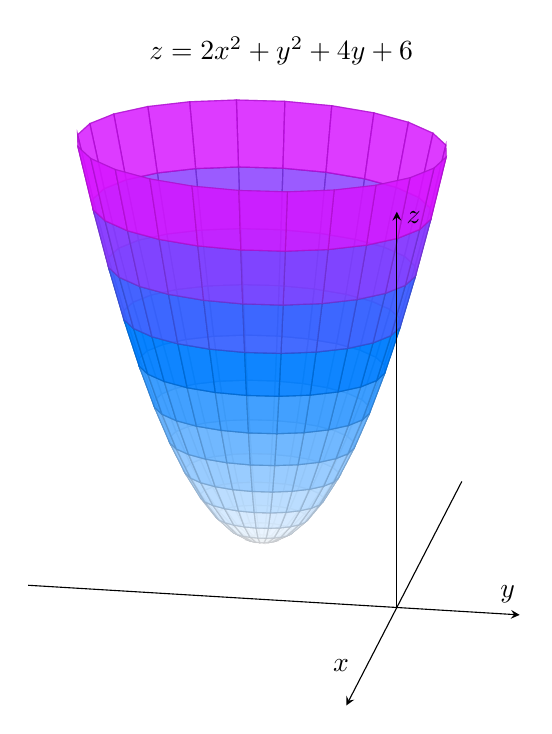
\begin{tikzpicture}
  \begin{axis}[
    title={$z=2x^2+y^2+4y+6$},
    title style={yshift=-10pt},
      view={100}{20},
      axis lines=center,
      axis equal image,
      xlabel={$x$},
      ylabel={$y$},
      zlabel={$z$},
      domain=0:2*pi,
      y domain=-2.25:2.25,
      samples=25,
      samples y=25,
      colormap/cool,
      axis on top,
      scale=1.5,
      xtick=\empty, ytick=\empty, ztick=\empty,
      z buffer=sort,
      xmin=-4.5, xmax=3.5,
      ymin=-4.5, ymax=1.5,
    ]
    \addplot3[
      surf,
      opacity=0.6
    ]
    ( {-2+(1/sqrt(2))*y*cos(deg(x))},
      {y*sin(deg(x))-2},
      {y^2} );
  \end{axis}
\end{tikzpicture}
\end{center}

\end{document}